\chapter{Análise e Desenho da Solução}
\label{sec:3-Analise}

Depois de contextualizados os temas relevantes, o presente capítulo foca-se na análise do problema 
que sustenta este relatório e na apresentação do desenho da solução criada.

\section{Domínio do Problema}

O fluxo que trata da informação de catálogo é dos mais sensíveis e cruciais para o bom funcionamento
dos sistemas que integram os serviços do grupo Flutter. Este fluxo funciona em tempo-real recorrendo
ao uso de \textit{streams} para conseguir atingir este objetivo. Esta abordagem permite garantir
o processamento assíncrono dos dados relativos a este fluxo de uma forma otimizada.

De momento, os serviços responsáveis pelo processamento destes dados estão distribuídos em dois
\glspl{cluster} que usam \textit{Apache Storm} para a gestão do mesmo. Esta solução apresenta algumas
limitações passíveis de análise por forma a melhorar a capacidade de escalabilidade destes serviços. 

A primeira destas limitações é o elevado número de \ac{VM} presente em cada \gls{cluster}. Este 
problema impacta a solução na fase de lançamento de novas versões. Isto deve-se ao facto de toda a 
infraestrutura estar sob demanda constante com vários lançamentos paralelos de vários serviços em 
ao ser necessário criar novas \ac{VM} o processo responsável pela gestão de máquinas da
infraestrutura pode não ser capaz de responder ao pedido. Desta forma, diminuir o número de \ac{VM}
presentes no \gls{cluster} representaria uma melhoria na probabilidade da taxa de sucesso de
lançamento de uma nova versão (em todos os ambientes).

Além disso, existem topologias presentes em certos \glspl{cluster} que estão a usar um excesso de
recursos face aos recursos que necessitam para operar sem falhas em alturas de pico de utilização
dos mesmos.

\subsection{Contexto}

O grupo Flutter é uma das maiores empresas de apostas desportivas a nível mundial. Este grupo
possui várias marcas que operam em diferentes mercados, como o mercado britânico, australiano e
norte-americano. A empresa tem vindo a crescer de forma exponencial nos últimos anos e, como tal,
tem vindo a investir em novas tecnologias e a expandir a sua presença em novos mercados. No mercado
de \ac{UKI} o grupo Flutter adquiriu, nos últimos meses uma nova marca - \ac{SBG} \cite{skybet}. 
Esta aquisição requer que os serviços necessários para a operação da marca dentro da infraestrutura 
do grupo seja migrada para a mesma. De momento, o \textit{hardware} disponível nos \glspl{dc} da 
empresa não é capaz de suprir as necessidades de processamento necessária para hospedar estes 
serviços, logo, é necessário levar a cabo um processo de otimização de recursos nos \glspl{cluster} 
existentes de forma a tornar possível que o serviço opere sem falhas.

\subsection{Modelo de Domínio}

Nesta secção vai ser apresentado o \ac{MD} simplificado do fluxo de catálogo disponibilizado nas 
plataformas de \textit{sportsbook} das empresas do grupo Flutter. A compreensão deste modelo será
importante para acompanhar a solução apresentada de seguida. A Figura \ref{md} apresenta a vista
simplificada deste modelo.

\begin{figure}[H]
  \centerline{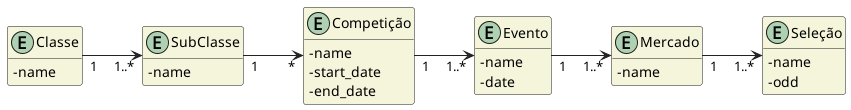
\includegraphics[scale=0.4]{media/content/analise/dm.png}}
  \caption{Modelo de Domínio - Fluxo de Catálogo (simplificado)}
  \label{md}
\end{figure}

De forma a ser mais simples acompanhar os termos apresentados na Figura \ref{md} vamos proceder 
a descrever uma hierarquia de exemplo:

\begin{itemize}
  \item \textbf{Classe} - Desporto (exemplo: Futebol)
  \item \textbf{SubClasse} - Especificação de Desporto (exemplo: Futebol Masculino)
  \item \textbf{Competição} - Competição (exemplo: Liga Portuguesa de Futebol)
  \item \textbf{Evento} - Evento (exemplo: FC Porto vs SC Espinho)
  \item \textbf{Mercado} - Tipo de Aposta (exemplo: Resultado Final)
  \item \textbf{Seleção} - Seleção de Aposta (exemplo: SC Espinho a vencer)
\end{itemize}

Como referido anteriormente, esta representação é apenas uma simplificação da realidade, isto
porque cada classe pode ter diferenças significativas na forma como representa a restante
hierarquia de relações entre entidades.

\section{Engenharia de Requisitos}

A Engenharia de Requisitos é uma área muito relevante no desenvolvimento de \textit{software}, pois 
sustenta a análise dos projetos, a primeira fase em que a equipa de desenvolvimento consegue 
compreender o domínio do negócio para o qual estão a desenvolver uma solução. Este passo representa 
o processo de obtenção de requisitos através de uma análise do problema e pressupõe a definição 
das necessidades, tanto por parte do cliente, como por necessidades técnicas, na procura de uma 
solução clara que valide a proposta apresentada. Seguindo um processo estruturado e adotando as 
melhores práticas, passamos a promover uma melhor comunicação entre as várias partes interessadas.

Considerando os aspetos mencionados, nesta secção serão apresentados os requisitos do sistema 
identificados e requisitados no início do projeto de maneira a garantir a que a solução desenvolvida 
vai de encontro com as necessidades apresentadas inicialmente. Estes requisitos podem ser 
categorizados em funcionais - funcionalidades distintas e essenciais que o sistema deve realizar, 
e não funcionais - restrições impostas para que o sistema realize os requisitos funcionais 
corretamente.

\subsection{Requisitos Não Funcionais}

Os requisitos não funcionais não se concentram no que o sistema faz, mas sim em como é esperado que
ele funcione. 

Os requisitos não funcionais apresentados de seguida, guiam-se pelo modelo FURPS+, um padrão de 
classificação qualitativa das características de um \textit{software} (\textbf{F}unctionality, 
\textbf{U}sability, \textbf{R}eliability, \textbf{P}erformance, \textbf{S}upportability), para 
facilitar a compreensão dos mesmos. O "\textbf{+}" refere-se a métodos de classificação diferentes, 
como por exemplo, restrições de design, implementação, interface ou físicos.

Estes requisitos são mais complexos de definir a nível do \gls{cluster}, pois cada topologia tem 
uma finalidade diferente, pelo que os requisitos são ligeiramente diferentes entre eles. De uma
forma geral, o sistema deve:

Para estes requisitos são definidos, para cada topologia, \acp{SLI} - os indicadores que mostram o
desempenho do sistema a todo o momento, \acp{SLO} - os objetivos que a equipa de desenvolvimento
deve atingir de forma a cumprir os \acp{SLA} - o acordo que o sistema mantém com os clientes a 
nível do seu funcionamento.

\vspace{5mm}

\textbf{Funcionalidade}
\begin{itemize}
  \item O sistema deve suportar a configuração de quatro ambientes de desenvolvimento - \ac{QA}, 
    desenvolvimento, performance e produção.
\end{itemize}

\textbf{Usabilidade}
\begin{itemize}
  \item Não aplicável.
\end{itemize}

\textbf{Fiabilidade}

\begin{itemize}
  \item O sistema deve ser capaz de recuperar de falhas de funcionamento sem perda de dados.
  \item O sistema deve ser capaz de recuperar de falhas de funcionamento automaticamente garantindo 
    o tempo de inatividade inferior a 1 minuto.
  \item O sistema deve ser capaz de recuperar de falhas de funcionamento sem intervenção manual.
\end{itemize}

\textbf{Desempenho}
\begin{itemize}
  \item O sistema deve manter a capacidade de processamento que tinha antes da intervenção.
  \item O sistema deve ser capaz de processar transações em dia de pico de catálogo \footnote[1]{
    Os "dias de pico de catálogo" são dias identificados previamente em que são criados muitos 
    eventos novos ou dias em que estão a ser realizados muitos eventos em simultâneo.}
    com atrasos de latência inferiores a 10 segundos.
\end{itemize}

\textbf{Suporte}
\begin{itemize}
  \item O sistema deve ter, pelo menos, 80\% de cobertura de testes unitários.
  \item O sistema deve ser validado por Engenheiros de \ac{QA} através de testes de integração e \ac{E2E}.
  \item O sistema deve suportar a replicação de \glspl{cluster} em dois \glspl{dc}.
\end{itemize}

\textbf{Restrições de Design}
\begin{itemize}
  \item O sistema deve suportar quatro ambientes - \ac{QA}, desenvolvimento, 
    performance e produção.
  \item O sistema deve estar replicado em dois \glspl{dc}.
  \item Todas as \ac{VM} do mesmo \gls{cluster} devem ter o mesmo \gls{flavour}.
  \item A paralelização deve ser feita por \ac{VM} e não por processo. Ou seja, a mesma \ac{VM} 
    não pode ter dois processos a correr em paralelo.
\end{itemize}

\subsection{Requisitos Funcionais}
\label{sec:3-rf}

Os requisitos funcionais especificam as unidades funcionais de um sistema de \textit{software}.
Estes requisitos concentram-se nas funções que devem ser disponibilizadas, descrevem as
funcionalidades, comportamentos e operações específicas que os utilizadores devem ser capazes de 
executar, podendo variar desde ações básicas, como entrada e saída de dados, a algoritmos 
específicos e processos de negócio.

É importante compreender estes requisitos de forma a garantir que a solução desenvolvida vai de
encontro com as necessidades apresentadas de um ponto de vista de negócio. Sem uma compreensão
clara destes requisitos, a solução desenvolvida pode não ser a mais adequada para o problema
e as otimizações efetuadas podem desvirtuar o objetivo do projeto.

De forma a facilitar a compreensão dos requisitos funcionais, estes encontram-se descritos na 
Tabela \ref{tab:reqfun} e na Figura \ref{dcu}, na forma de \textit{User Stories}.

\begin{table}[H]
  \begin{center}
    \caption{Requisitos Funcionais}
    \vspace{5mm}
    \label{tab:reqfun}
    \begin{tabular}{|c|l|}
      \hline
      ID & User Story                                                                  \\ \hline
      1  & \begin{tabular}[c]{@{}l@{}}Como utilizador, pretendo consultar os eventos ativos \\
        num determinado dia. \\
      \end{tabular} \\ \hline
        2  & \begin{tabular}[c]{@{}l@{}}Como utilizador, pretendo consultar os tipos de aposta \\
        disponíveis para um determinado evento. \\
      \end{tabular} \\ \hline
        3  & \begin{tabular}[c]{@{}l@{}}Como utilizador, pretendo consultar as \glspl{odd} de um\\
        num determinado evento. \\
      \end{tabular} \\ \hline
    \end{tabular}
  \end{center}
\end{table}

\begin{figure}[H]
  \centerline{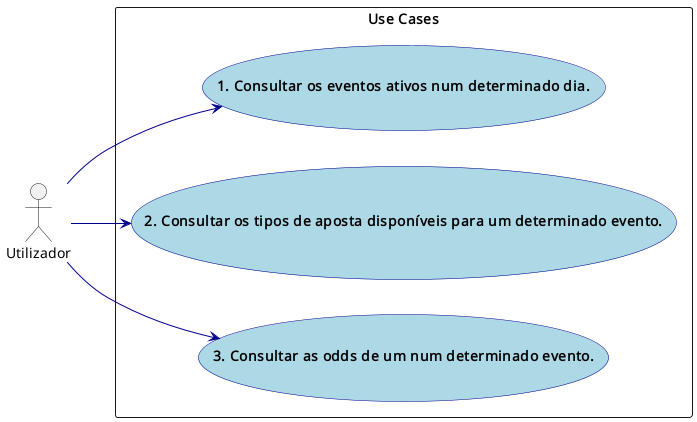
\includegraphics[scale=0.4]{media/content/analise/ucd.png}}
  \caption{Diagrama de Casos de Uso}
  \label{dcu}
\end{figure}

\section{Estado Atual do Sistema}

O sistema em análise é composto por vários \glspl{cluster} que suportam os serviços de catálogo
disponibilizados pelas marcas do grupo Flutter. Estes \glspl{cluster} são compostos por várias
\ac{VM} que executam as topologias responsáveis pelo processamento dos dados relativos a estes
serviços. A Tabela \ref{tab:current_setup} apresenta o estado atual dos \glspl{cluster}.

O número de \ac{CPU} apresentado representa o número de \ac{CPU} dedicados a cada \ac{VM}. Na
última linha da tabela são apresentados os números de \ac{VM} "usadas" e \ac{VM} "totais" que são,
respetivamente, o número de \ac{VM} que é necessário para as topologias conseguirem operar e 
o número de \ac{VM} que são disponibilizadas realemente no \gls{cluster} de forma a garantir a 
resiliência e recuperação em caso de falhas.

\begin{table}[H]
  \centering
  \begin{tabular}{|l|l|l|l|l|}
    \cellcolor{white} & \multicolumn{2}{|c|}{\cellcolor[HTML]{FBE6A3}\textbf{Estado atual}}                              \\ \cline{1-4} 
    & \cellcolor[HTML]{4EAC5B}Cluster 1 - 8cpu16GB          & \cellcolor[HTML]{4EAC5B}Cluster 2 - 6cpu12GB          &                            \\ \cline{1-4} 
    & \cellcolor[HTML]{A9D08E}ELR * 2                       & \cellcolor[HTML]{BDD7EE}TMT                           &                            \\ \cline{1-4} 
    & \cellcolor[HTML]{A9D08E}ELM * 2                       & \cellcolor[HTML]{BDD7EE}IMG\_EMT                      &                            \\ \cline{1-4} 
    & \cellcolor[HTML]{A9D08E}BFP                           & \cellcolor[HTML]{BDD7EE}FHG                           &                            \\ \cline{1-4} 
    & \cellcolor[HTML]{A9D08E}BETRADAR                      & \cellcolor[HTML]{BDD7EE}DOS                           &                            \\ \cline{1-4} 
    & \cellcolor[HTML]{A9D08E}PBT * 2 * 5                   & \cellcolor[HTML]{BDD7EE}CM * 2 * 5                    &                            \\ \cline{1-4} 
    & \cellcolor[HTML]{A9D08E}ESL * 2                       & \cellcolor[HTML]{BDD7EE}LMT * 2                       &                            \\ \cline{1-4} 
    & \cellcolor[HTML]{A9D08E}EventType * 2                 & \cellcolor[HTML]{BDD7EE}EXT                           &                            \\ \cline{1-4} 
    & \cellcolor[HTML]{A9D08E}FIP * 2 * 5                   & \cellcolor[HTML]{BDD7EE}ET                            &                            \\ \cline{1-4} 
    & \cellcolor[HTML]{A9D08E}HKR * 2                       & \cellcolor[HTML]{BDD7EE}MTT * 2                       &                            \\ \cline{1-4} 
    &                                                       & \cellcolor[HTML]{BDD7EE}PBS * 2                       &                            \\ \cline{1-4} 
    &                                                       & \cellcolor[HTML]{BDD7EE}SGM * 3                       &                            \\ \cline{1-4} 
    &                                                       & \cellcolor[HTML]{BDD7EE}IMG\_LDT                       &                            \\ \cline{1-4} 
    &                                                       & \cellcolor[HTML]{BDD7EE}TPD                           & Total                      \\ \cline{1-4}
    \cellcolor[HTML]{C0C0C0}CPU                             & 1280                                                     & 432                                                     & \textbf{1712}                 \\ \cline{1-4}
    \cellcolor[HTML]{C0C0C0}RAM                             & 2560                                                    & 864                                                     & \textbf{3424}                \\ \cline{1-4}
    \cellcolor[HTML]{C0C0C0}Used VM                         & 160                                                     & 72                                                      & \textbf{232}                 \\ \cline{1-4}
    \cellcolor[HTML]{C0C0C0}Total VM                        & 185                                                     & 77                                                      & \textbf{262}                 \\ \cline{1-4}
  \end{tabular}
  \caption{Estado atual dos \textit{clusters}}
  \label{tab:current_setup}
\end{table}

\subsection{Balanceadores de Carga}

Para lidar com falhas e garantir a disponibilidade dos serviços, os serviços de catálogo estão
distribuídos por dois \glspl{dc} e o tráfego de entrada é distribuído por um \ac{LB} que encaminha
o tráfego para os \gls{cluster} do \ac{DC} escolhido. Já a nível do \gls{cluster}, a gestão de 
tráfego e falhas é gerida pelo próprio \textit{Apache Storm} que garante a replicação dos dados
e a recuperação de falhas entre as réplicas de cada topologia.

De forma a simplificar a compreensão destes conceitos, a Figura \ref{lb} apresenta um diagrama
simplificado da arquitetura de \ac{LB} presente nos \glspl{cluster}, sendo que a gestão efetuada
a nível do \textit{Apache Storm} é simplificada como um \ac{LB} interno.

Na realidade, esta gestão por parte do Apache Storm é mais complexa, pois usa o conjunto de
máquinas que tem disponível para paralelizar o processamento realizado por parte das topologias e
recuperar de falhas.

\begin{figure}[H]
  \centerline{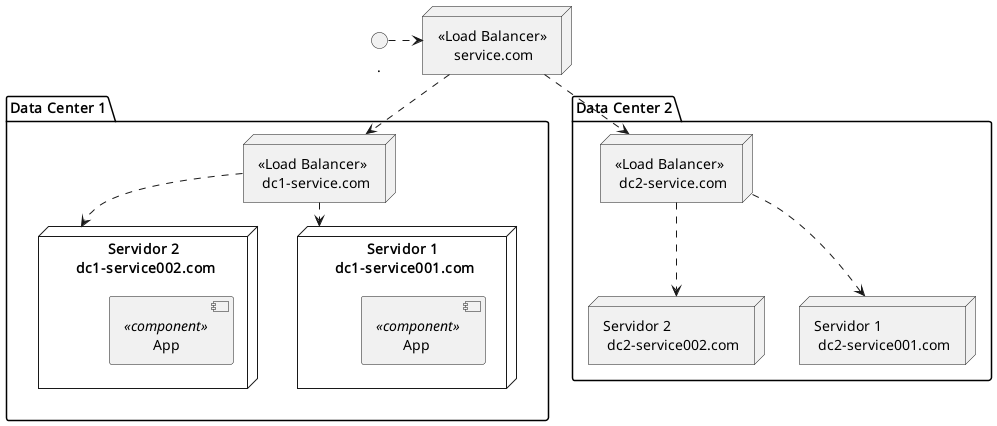
\includegraphics[scale=0.45]{media/content/analise/lb.png}}
  \caption{Arquitetura dos Balanceadores de Carga}
  \label{lb}
\end{figure}

Como ilustrado na Figura \ref{lb} todo o sistema de balanço de carga é abstraído do utilizador
final através da atribuição do \ac{DNS}. Ao fazer um pedido ao endereço \textit{service.com} a primeira
camada de balanço de carga decide qual é o \ac{DC} que vai ficar encarregue de processar o pedido,
esta escolha pode seguir diversas estratégias como proximidade geográfica ao cliente que está a 
efetuar o pedido, a disponibilidade atual do \ac{DC}, entre outras. De seguida, um dos 
balanceadores de carga de um dos \ac{DC} vai receber o pedido e repetir o processo para definir
qual é a máquina que vai ficar encarregue por processar realmente o pedido do utilizador.

\subsection{Análise de Uso de Recursos}

A primeira fase do desenho da solução passa pela análise do uso de recursos dos \glspl{cluster}
que suportam os serviços de catálogo. Para tal, foram analisadas duas janelas temporais distintas
onde os serviços sofreram uma carga acima do normal. Desta forma, é possível ter uma visão clara
das possíveis otimizações de recursos a fazer já que o objetivo final é que o \gls{cluster}
mantenha a sua capacidade de processamento e seja capaz de suportar a mesma carga a que estava
sujeito antes desta intervenção.

Para isso, é importante, em primeiro lugar, compreender a forma como estes serviços são requisitados
pelo sistema para, desta forma, ser possível analisar o intervalo de datas correto. Neste caso,
todos os serviços disponibilizados pelos \glspl{cluster} são relativos ao catálogo, ou seja,
à informação relativa aos vários eventos disponibilizados aos clientes. Desta forma, os intervalos
a analisar devem ser períodos em que sejam criados muitos eventos novos, ou momentos em que
estejam a ser realizados vários eventos em simultâneo e o sistema de atualização de \glspl{odd}
esteja a ser bastante utilizado.

Após discussão com vários elementos mais experientes no negócio concluiu-se que os intervalos
adequados a esta análise seriam em agosto - quando são criados os eventos relacionados com as
principais ligas dos maiores desportos a nível europeu, como futebol e basquetebol - e dezembro 
quando existe uma nova vaga de criação de eventos nesses desportos e também a disponibilização 
dos calendários noutros desportos disponíveis nas plataformas de \textit{sportsbook} como
corridas de cavalos.

Para a análise destes dados foram usadas as métricas disponibilizadas no \textit{Grafana}. Em alguns
casos foi necessário a criação de novos \textit{dashboards} para a análise de métricas mais 
específicas para cada serviço, mas na maioria dos casos as métricas mais relevantes eram métricas 
de sistema, como uso de processador e de memória RAM.

Esta análise foca-se no uso de recursos de cada topologia. Na Figura \ref{analise-ofs} podemos
analisar o uso de recursos de um dos \glspl{cluster}. A restante análise encontra-se
presente em no Anexo \ref{appendix-a}.

Em cada linha desta tabela está presente uma topologia e as várias métricas a nível de uso de 
recursos de \textit{hardware} nos períodos identificados como "dias de pico", neste caso, um dia 
do mês de agosto e um dia no final do ano. Ao analisar os recursos de \ac{CPU} e memória RAM de 
cada topologia nestes períodos podemos extrapolar um majorante do uso de recursos necessários para
esta topologia poder operar sem falhas no dia mais exigente do ponto de vista computacional no ano.

\begin{figure}[H]
  \centerline{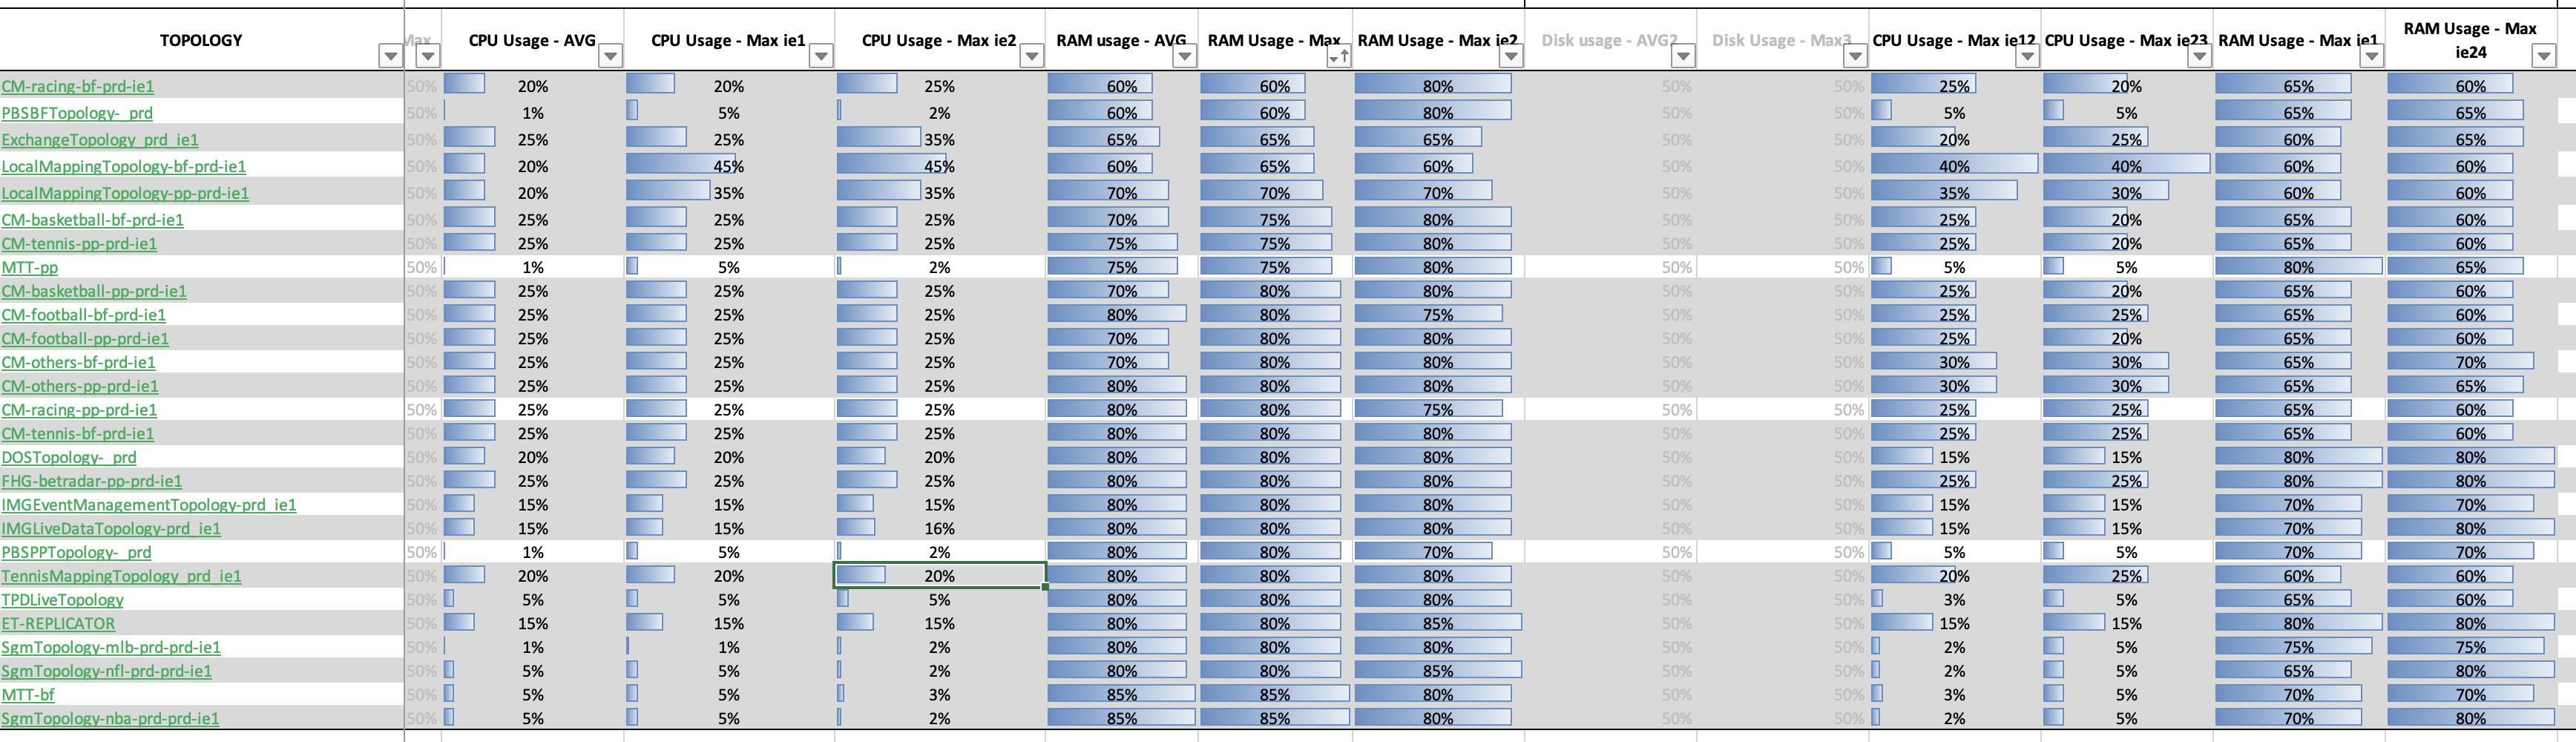
\includegraphics[scale=0.27]{media/content/analise/analise-ofs.png}}
  \caption{Análise do uso de recursos de um dos \textit{clusters}}
  \label{analise-ofs}
\end{figure}

Através da análise dos campos de uso máximo de \ac{CPU} e memória RAM de cada topologia, é possível
extrapolar o \gls{flavour} de \ac{VM} que cada topologia necessita para operar sem falhas.

Esta análise permitiu concluir que existem topologias que estão hospedadas num \gls{cluster}
com um \gls{flavour} superior ao que necessitam para processar a carga que lhes é atribuída,
mesmo em momentos de pico. 

